\msusection{Preferences}\label{sec:pref}
YCweather offers a variety of customizable options for controlling how the program operates.  These options are available in the Preferences, which may be opened via the Program Control File menu or with the Toolbar button.  Figure \ref{fig:pref} shows the Preferences window.  This window is divided into three parts, each of which has a number of options as discussed below.

\begin{figure}[h]\centering
	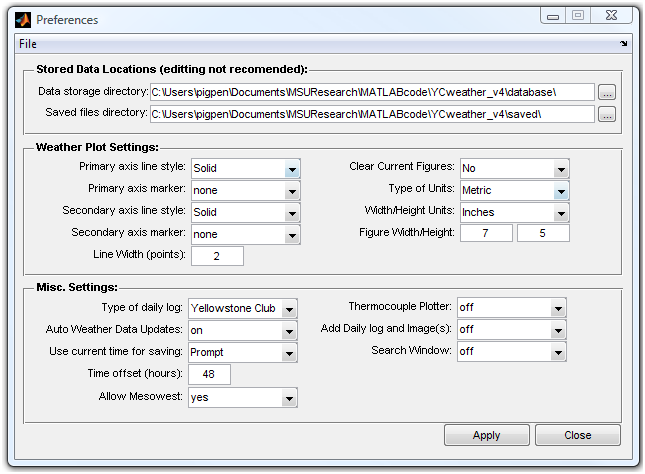
\includegraphics[width=\linewidth]{\YCfiles figures/pref.png}
	\caption{YCweather preferences window.}
	\label{fig:pref}
\end{figure}

In order for the changes in preferences to take place, the Apply button must be pressed.  The changed setting will only apply to the current YCweather workspace and will return to the default settings when YCweather is reopened.  The selected preferences may be defined as the default by selecting the Set Default option in the Preferences window File menu.  Additionally, if the workspace is saved (Section \ref{sec:workspace}) the current setting are applied to that workspace file and will remain when this workspace is opened in subsequent executions of this workspace file.

\msusubsection{Stored Data Locations}
As indicated in the Preferences window (Figure \ref{fig:pref}) editing the \q{database} and \q{saved} directory is not recommended unless a thorough understanding of file structure of YCweather is possessed.  These details are included in Section \ref{sec:advanced}, which discuss how YCweather operates. The \q{database} directory is where all the weather data, images, and log files are stored.  And the \q{saved} directory is the default location for all YCweather related files created by the user.

\msusubsection{Weather Plotting Settings}
The left-hand column in this section controls how the lines of weather graphs will appear upon creation, allowing for the adjustment of the line style, line markers, and line width for both the primary (left-side) and secondary (right-side) axes. The right-hand column includes various options, which are summarized in the following list.
\begin{itemize}
     \nitem{Clear Current Figures:} If this value is set to \q{Yes} then each time a graph is created all others are deleted.
     \nitem{Type of Units:} Specifies the units to display when graphs are created.  Note, if this is changed a new Data List window must be created because the unit conversion occurs during the creation of this window.
     \nitem{Width/Height Units:} Sets the units of the graph size upon creation, the numeric value for this setting is provided in the following item.
     \nitem{Figure Width/Height:} The width and height of a graph created based on the units specified above.
\end{itemize}

\msusubsection{Misc. Settings}
The settings in Misc. Settings panel, as the name suggests,  control various aspects of YCweather.  The first three items in the right-hand column toggle the appearance of the corresponding side panels when YCweather opens.  These panels are detailed in Section \ref{sec:panels}. 

The left-hand column allows the user to determine the type of daily log that YCweather should utilize, see Section \ref{sec:dailylogs} for details.  The Auto Weather Data Update options toggles the automatic download of the latest available weather data, as detailed in Section \ref{sec:data}.  The next  two options in this column control the graphing start and end times when graphs are created via workspaces, which is discussed in Section \ref{sec:workspace}. Finally, the ``Allow Mesowest'' setting toggles the capability for YCweather to communicate with the \href{http://mesowest.utah.edu/index.html}{MesoWest} database, which requires Internet access. Additional details regarding the \href{http://mesowest.utah.edu/index.html}{MesoWest} feature may be found in Section \ref{sec:mesowest}.
